\documentclass{beamer}

\usetheme{Malmoe}
\usecolortheme{spruce}

\usepackage{amsmath,amsthm,amssymb}
\usepackage{mathtools}
\usepackage{mathrsfs}
\usepackage{enumitem}
\usepackage{physics}

\newcommand{\avg}[1]{\left<#1\right>}

%Information to be included in the title page:
\title{The Top Quark}
\author{Sean Ericson}
\institute{UO}
\date{}
\titlegraphic{
\includegraphics[scale=0.75]{images/seal.jpg}}

\begin{document}

\frame{\titlepage}

\begin{frame}
\frametitle{History (prediction)}
\begin{itemize}
    \item<1-> 1973: Makoto Kobayashi and Toshihide Maskawa propose expanding the then known quark quartet to a 6-plet to explain CP-violating weak interactions
    \begin{center}
        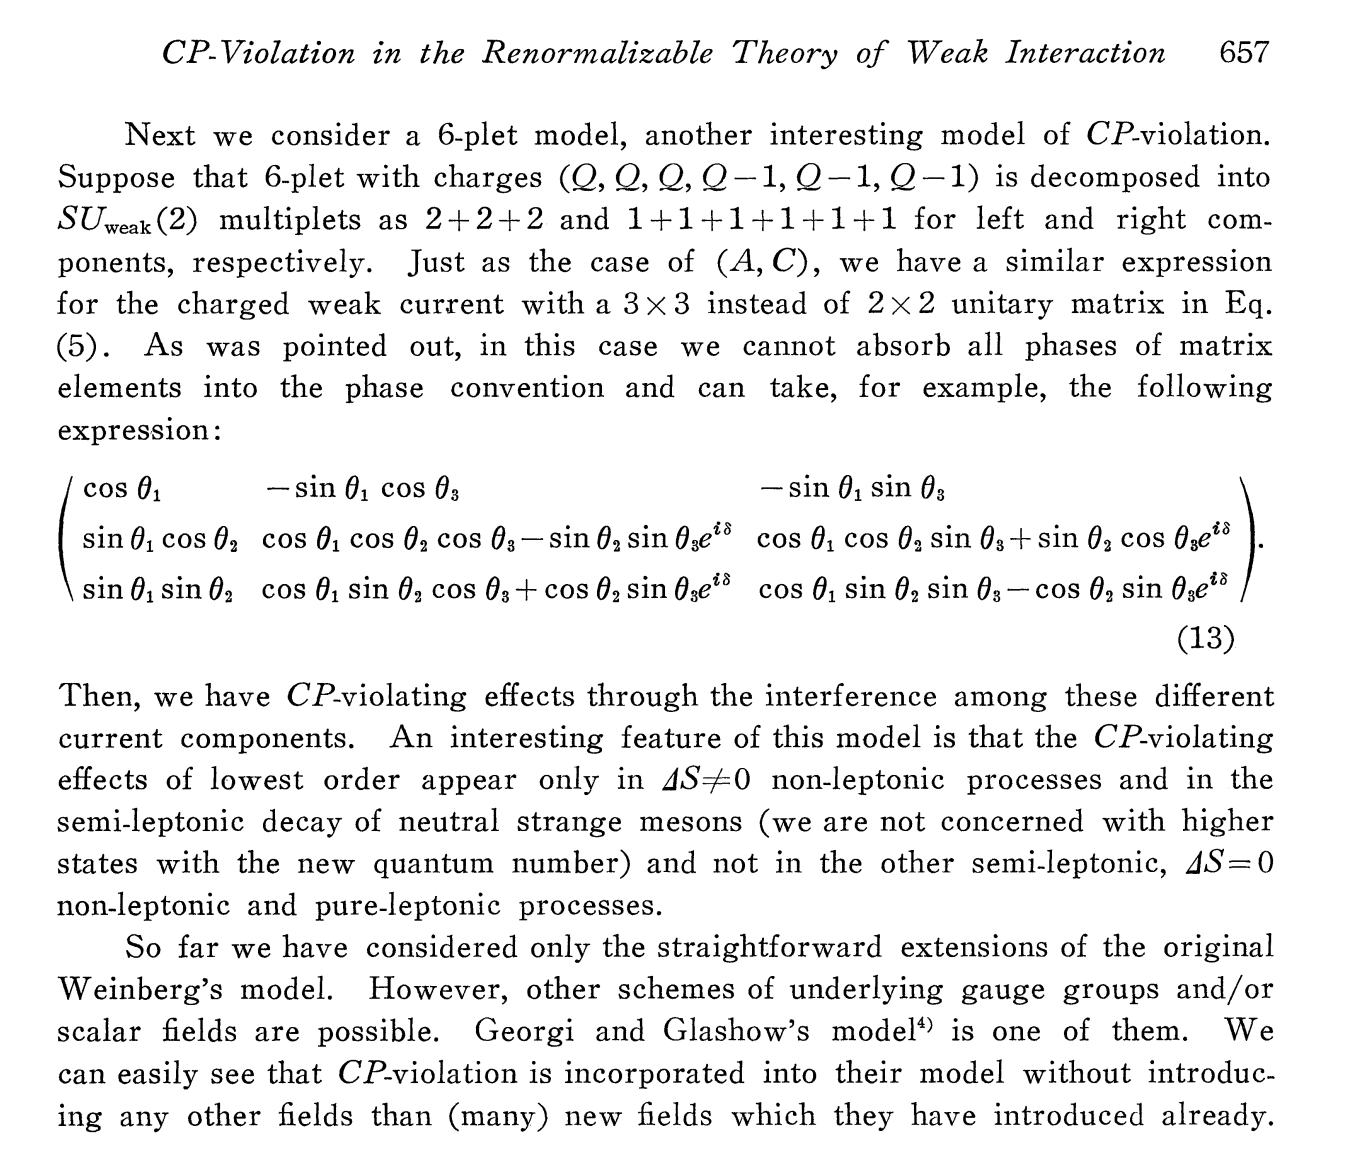
\includegraphics[scale=0.3]{images/6plet.PNG}
    \end{center}
\end{itemize}
\end{frame}

\begin{frame}
\frametitle{History (prediction)}
    \begin{itemize}
        \item<1-> 1975: Haim Harari proposes the names "Top" and "Bottom" for the additional quarks.
        \begin{center}
            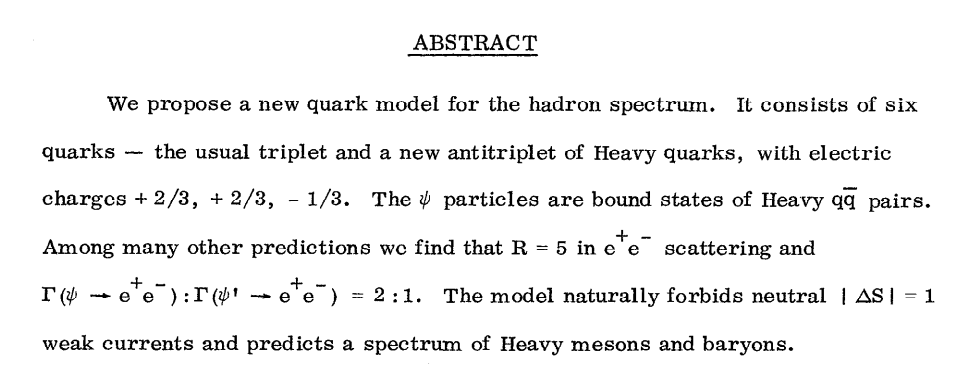
\includegraphics[scale=0.6]{images/harari.PNG}
        \end{center}
    \end{itemize}
\end{frame}

\begin{frame}{History (discovery)}
    \begin{itemize}
        \item<1-> 1995: Nearly 20 years later, the Top is discoverd at Fermilab by the CDF and D0 collaborations.
        \begin{center}
            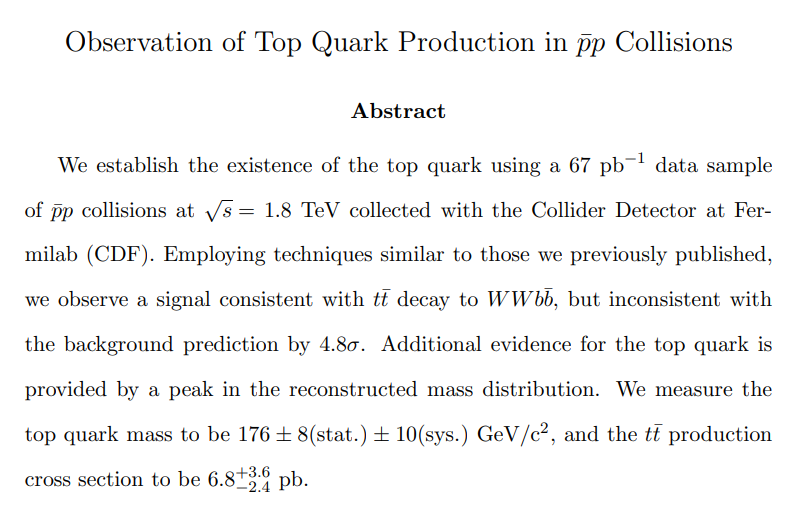
\includegraphics[scale=0.35]{images/cdf.PNG}
            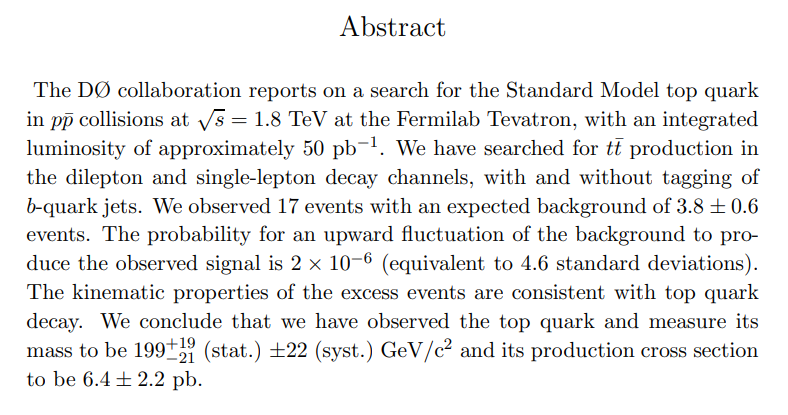
\includegraphics[scale=0.35]{images/D0.PNG}
        \end{center}
    \end{itemize}
\end{frame}

\begin{frame}{Asside: Major Particle Discoveries}
    \begin{itemize}
        \item<1-> 1937/1947: The $\mu$/$\pi$ mess-up 
        \item<2-> 1947: The K meson
        \item<3-> 1950: The $\Lambda$ baryon
        \item<4-> 1964: The $\Omega$ and $\Xi$ baryons
        \item<5-> 1969: up, down, and strange quarks (as partons)
        \item<6-> 1974: The J/$\Psi$ meson
        \item<7-> 1975: The $\tau$ lepton
        \item<8-> 1979: the gluon
        \item<9-> 1983: The W and Z bosons
        \item<10-> 1995: The top quark (finally!)
        \item<11-> 2012: The higgs boson
    \end{itemize}
\end{frame}

\begin{frame}{Properties}
    \begin{itemize}
        \item<1-> The top quark was found to have a mass of roughly 170 GeV! For reference, that's
        \begin{itemize}
            \item<2-> 1.4 x the mass of the higgs
            \item<3-> 1.9 x the Z mass
            \item<4-> 0.89 x the mass of a $\text{Pb}^{208}$ atom
            \item<5-> 0.96 x the mass of a caffeine molecule! 
        \end{itemize}
        \item<6-> The decay width of the top, $\Gamma \approx 1.4 GeV$ corresponds to a lifetime $\tau \approx 5\times 10^{-25}$ s.
        \begin{itemize}
            \item<7-> That's about $10^{15}$ times shorter than the Cesium hyperfine transition period used to define the second!
            \item<8-> In that time, light travels about 0.15 fm.
        \end{itemize}
    \end{itemize}
\end{frame}

\begin{frame}{Properties (theoretical mass constraints)}
    \begin{itemize}
        \item<1-> Measurements of processes that don't directly involve the top quark can help place theoretical constraints on the top quarks mass.
        \begin{itemize}
            \item<2-> Virtual top quarks can appear in radiative corrections to some processes.
            \item<3-> Example: flavor oscillation in neutral $\text{B}_\text{s}^0$ mesons:
        \end{itemize}
        \begin{center}
            \includegraphics<3->[scale=0.25]{images/B_oscillation.png}
        \end{center}
        \item<4-> Beyond Standard Model theories also constrain the mass of the top quark.
    \end{itemize}
\end{frame}

\begin{frame}{Production ($t\bar{t}$-pairs)}
    \begin{itemize}
        \item<1-> The primary processes that produce top quarks in colliders are $q\bar{q} \to t\bar{t}$ and $gg \to t\bar{t}$.
        \item<2-> $t\bar{t}$ pair production is a strong-force interaction.
        \begin{itemize}
            \item<3-> ~85\% of the cross section at the Tevatron is from $q\bar{q}$ annihilation ($p\bar{p}$ @ $\sqrt{s}$ = 1.96 TeV)
            \item<4-> ~90\% of the cross section at the LHC is from gluon fusion ($pp$ @ 14 TeV)
        \end{itemize}
        \begin{center}
            \includegraphics<5->[scale=0.35]{images/top_pair_production_diagrams.PNG}
        \end{center}
    \end{itemize}
\end{frame}

\begin{frame}{Production ($t\bar{t}$-pairs)}
    \begin{center}
        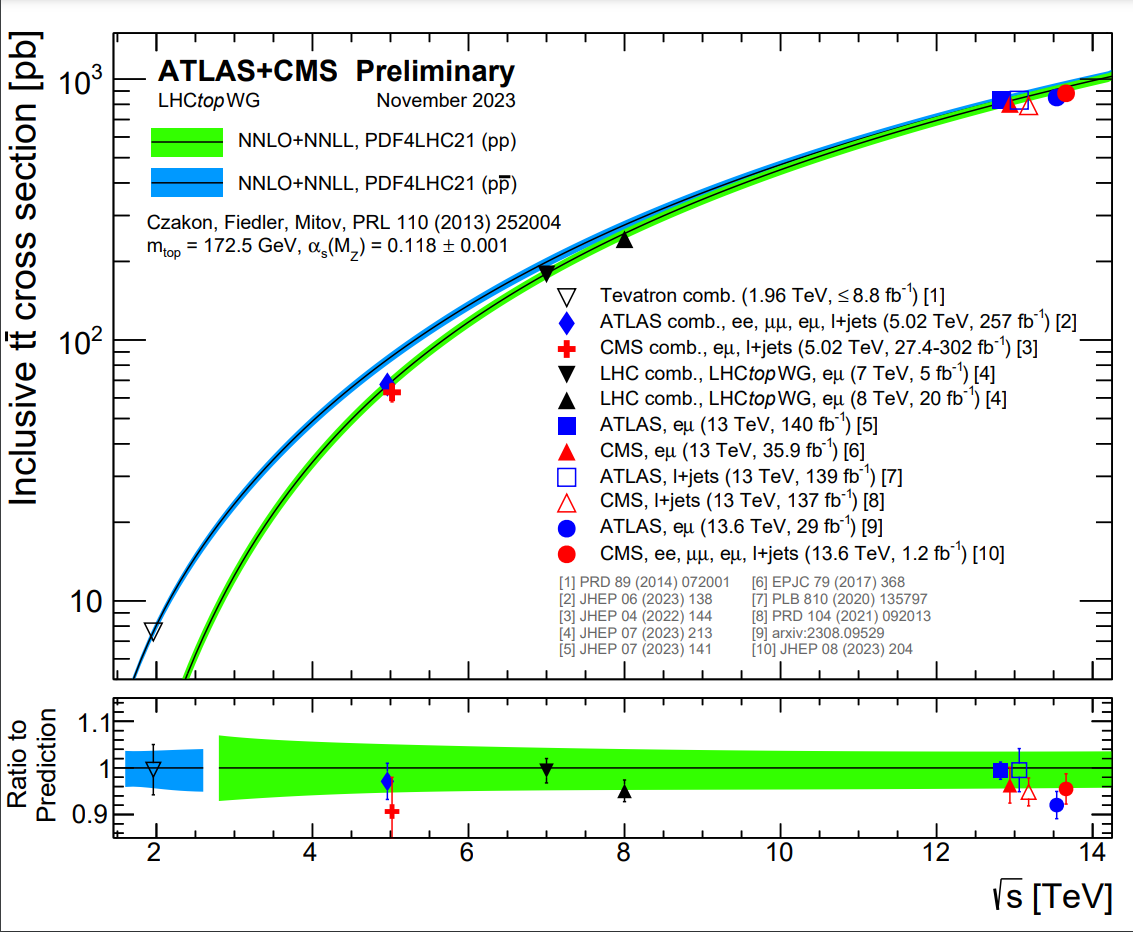
\includegraphics[scale=.45]{images/top_pair_production_cross_section.PNG}
    \end{center}
\end{frame}

\begin{frame}{Production (single top)}
    \begin{itemize}
        \item<1-> Much more rarely, single tops are produced through weak interactions.
        \begin{center}
            \includegraphics<2->[scale=0.35]{images/single_top_production_diagrams.PNG}
        \end{center}
        \item<3-> t-channel processes, though suppressed by the week interaction, are kinematically enhanced.
        \item<4-> t- and s-channel production rates at the Tevatron are identical for $t$ and $\bar{t}$, but different at the LCH due to initial state charge asymmetry.
        \item<5-> In the limit $\abs{V_{tb}} \gg \abs{V_{td}}, \abs{V_{ts}}$ single top production cross sections are proportional to $\abs{V_{tb}}^2$
    \end{itemize}
\end{frame}

\begin{frame}{Decay}
    \begin{itemize}
        \item<1-> Top quarks decay through the weak interaction.
        \begin{itemize}
            \item<2-> Primarily into a W boson and bottom quark (~95\% of the time)
        \end{itemize}
        \item<3-> The decay width is also proportional to $\abs{V_{tb}}^2$.
        \includegraphics<4->[scale=1]{images/width_calc.PNG}
        \item<5-> Exotic decay modes involving the production of a Z boson and a charm or up quark are theoretically possible, but have never been observed.
    \end{itemize}
\end{frame}

\begin{frame}{Decay}
    \begin{center}
        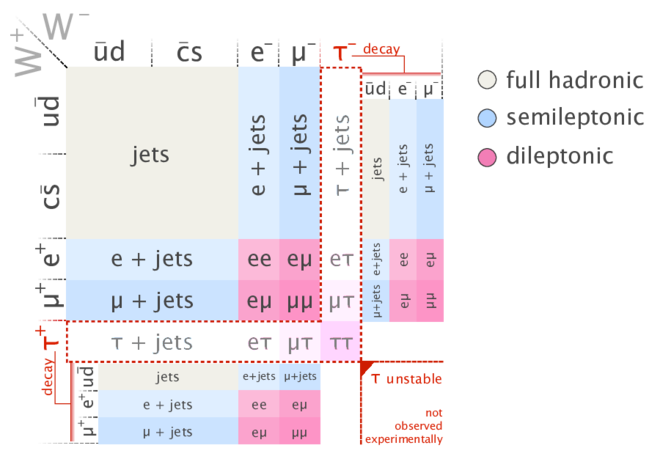
\includegraphics[scale=0.4]{images/decay_types.png}
    \end{center}
\end{frame}

\begin{frame}{Decay}
    \begin{center}
        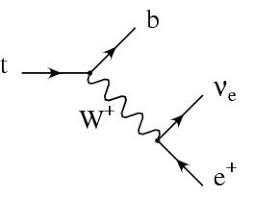
\includegraphics[scale=0.5]{images/decay.jpg}
    \end{center}
\end{frame}

\begin{frame}{Higgs Production}
    \begin{center}
        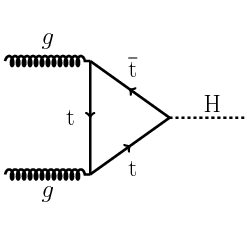
\includegraphics[scale=1]{images/higgs.png}
    \end{center}
\end{frame}

\end{document}